\section{MAC}

Goal: Resource-efficient collision avoidance. Scalable, robust and fair.
Collisions and overhearing cause lots of energy loss, so should be avoided.

\begin{description}
		\item[Scheduled protocols]: Polling (central controller allocates
				slots) vs multiplexing (pre-allocated channels), but causes
				overhead (polling) or not scalable (multiplexing)
		\item[Contention-based protocols] On-demand sharing of channels, but
				inefficient in times of contention
		\item[Hybrid approaches] Combining scheduled and contention-based
\end{description}

\subsection{Scheduled protocols}

Access scheduled. Collision-free, but costly to maintain, requires synchronized
nodes.

\subsubsection{Based on clustesr}

Idea: Form clusters, one node acts as cluster head and schedules access. Nodes
only communicate with cluster head.

\paragraph{Low Energy Adaptive Clustering Hierarchy, LEACH}

\begin{itemize}
		\item Nodes organize into clusters with rotating heads. Only active
				when transmitting.
		\item Cluster heads always active. Calculate schedule for nodes,
				aggregate data and forward to sink.
		\item Cluster head election once per round. Each nodes elects self with
				certain probability, dependant on e.g. energy level. Other
				nodes then join cluster head with strongest signal.
\end{itemize}

\subsubsection{Self-organizing}

\begin{itemize}
		\item Nodes find each other on fixed frequency, agree on pair of slots
				to transmit and receive. Leads to a frequency/time/mode tuple
				for each pair of nodes.
\end{itemize}

\subsubsection{Lightweight MAC}

\begin{itemize}
		\item Time-based multiplexing, based on choices of 1-hop neighbours
\end{itemize}

\subsection{Contention-based protocols}

Shared channels. ALlocation on demand. Flexible and scalable, no need for
synchronicity, but potentially inefficient when there is contention.

\subsubsection{Wakeup radio}

\begin{itemize}
		\item Idle channel randomly chosen. If no idle channel available, random backoff.
		\item Low-power control channel indicates upcoming transmission, wakes
				nodes from sleep if they are destination.
\end{itemize}

\subsubsection{Periodic wakeup}

\begin{itemize}
		\item Receiving node periodically wakes up. Requires sending node to know about duty cycles.
		\item Or sending node must announce transmission ahead of time
		\item Or send long preamble (> sleep cycle)
		\item Or receiving node announces its wake time
		\item Or time synchronization
\end{itemize}

\begin{description}
		\item[X-MAC] Preamble including address, receiver acks preamble, then data follows
		\item[BEAM] Long or short preambles with/without payload. Receiver acks
				preamble (if without payload) or full data frame (if with
				payload). Preamble in the front allows non-intended receivers
				to sleep early.
		\item[B-MAC] Long preamble followed by data. Receiver periodically
				wakes to listen for preamble.
		\item[WiseMAC] Sender sends preamble prior to data packet, nodes
				periodically check medium. If medium busy, they receive. Nodes
				tell each other about sampling schedule via ACKs.
		\item[ContikiMAC] Combination of B-MAC (low-power listening), X-MAC
				(preamble), BEAM (data packets), WiseMAC (receiver wakeup time
				estimation)
		\item[Maximally Traffic-Adaptive and energy-efficient MAC] Sampling of
				preambles like WiseMAC, change sampling frequency by frequency
				of recently received packets.
		\item[Receiver-initiated MAC] Source becomes active, listens to
				destination's beacon. Once received it sends data. Destination
				acks.
		\item[Sensor MAC] Each node picks and periodically broadcasts its
				sleep/listen schedule. If it receives another's schedule it
				adopts it. If no other neighbours it adopts it exclusively, if
				other neighbours then it attempts following both.
		\item[Traffic-aware energy-efficient MAC] Optimizes S-MAC by combining
				SYNC and RTS.
\end{description}

Max-MAC:
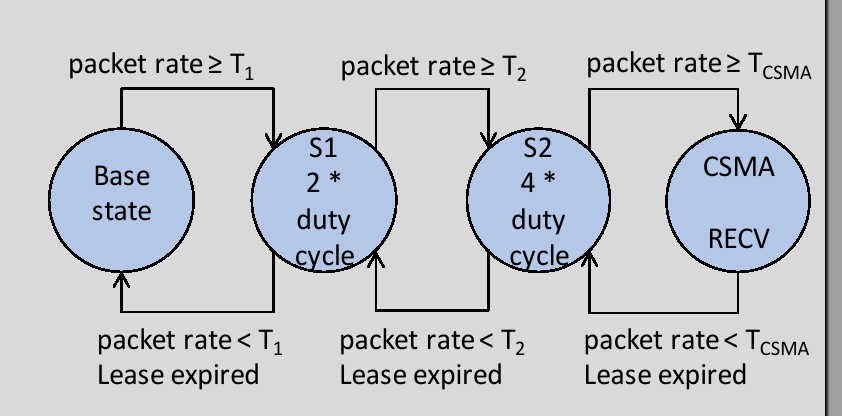
\includegraphics[width=0.5\textwidth]{07_max_mac}

Sensor MAC
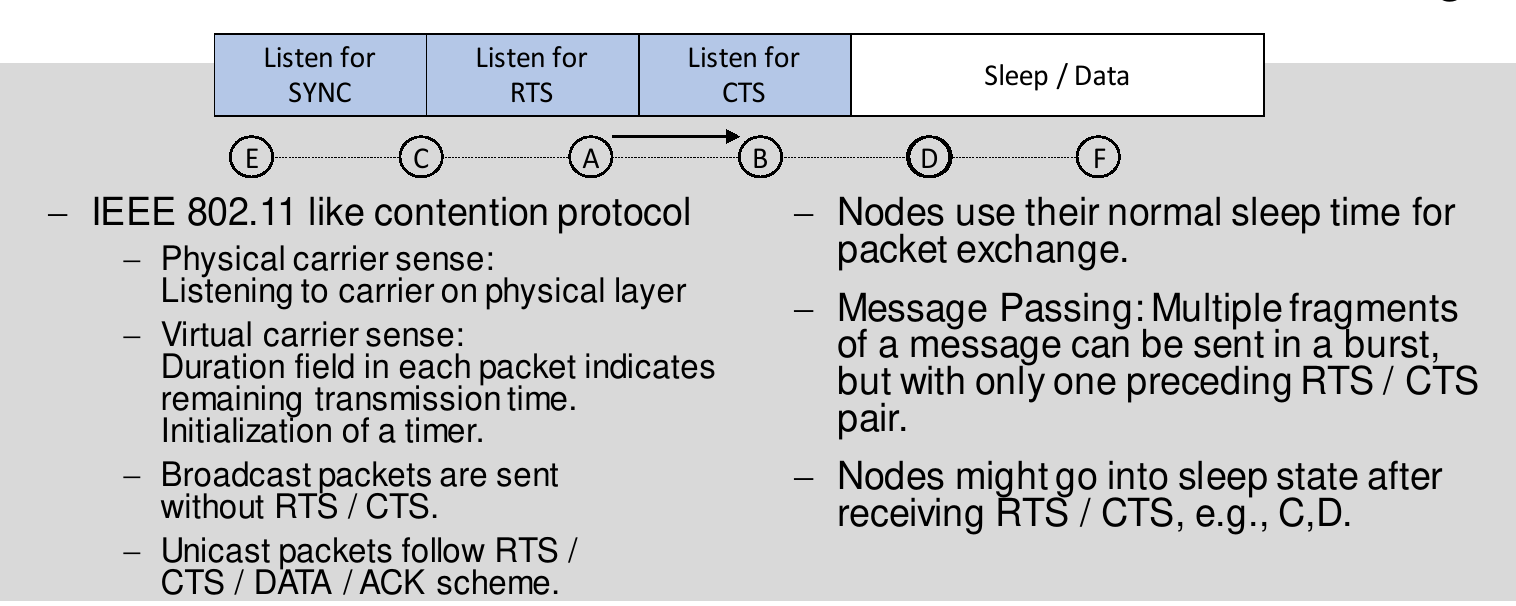
\includegraphics[width=\textwidth]{07_smac}

\subsection{Industry standards}

\subsubsection{IEEE 802.15.43, Low-rate wireless PAN}

Specifies wireless MAC and physical layer for low-rate WPAN. Contiki only uses
physical layer, not MAC layer. Standard is basis for e.g. ZigBee and WirelessHART.

\begin{itemize}
		\item OTA data rates of up to \SI{250}{kbps}
		\item Optional allocation of guaranteed time slots
		\item Carrier-sense multiple access with collision avoidance
		\item Link quality indication
		\item Two types of device: Full-function which can operate as
				coordinator. Reduced-function, which only works as device.
		\item FFD can talk to RFD and FFD, RFD only to FFD.
		\item Forms tree-like structures with RFDs in leaves, FFDs in other
				places.
\end{itemize}

\paragraph{Slot structure}

Coordinator defines slots. Some for contention-based access (with e.g.
listening), some with guaranteed (scheduled) access. Part of the superframe can
also be empty, allowing coordinator to sleep.

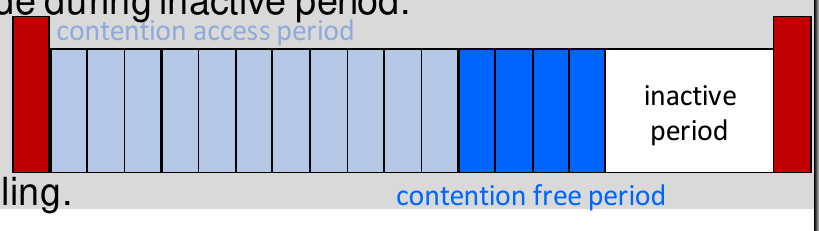
\includegraphics[width=0.5\textwidth]{07_ieee}

\paragraph{Low-energy mechanisms}

\begin{description}
		\item[Coordinated sampled listening] Receiving and transmitting devices
				coordinate sampling times to reduce overhead.
		\item[Receiver-initiated transmission] Receiving devices beacon data
				request, transmitting devices only transmit when such a beacon
				received.
\end{description}

\subsubsection{Wireless HART}

\begin{itemize}
		\item Fore wireless sensor networks, based on IEEE 802.15.4 physical layer
		\item TDMA MAC with rigid time synchronization requirement across entire network
		\item \SI{10}{ms} slots
\end{itemize}

\subsubsection{LoraWAN}

\begin{itemize}
		\item Secure bidirectional communication
		\item Star-of-stars topology
		\item End devices use single-hop communication to one or many gateways
		\item LoraWAN network server manages data rate and RF output of each end-device
\end{itemize}

Three types of devices:

\paragraph{Class A, battery powered}

\begin{itemize}
		\item Picks its own transmission slot, with small random variation
		\item Opens two receive windows
\end{itemize}

\paragraph{Class B, low latency}

\begin{itemize}
		\item Scheduled receive slots assigned by beacon from gateway
		\item Unicast and multicast
\end{itemize}

\paragraph{Class C, no latency}

\begin{itemize}
		\item Nearly continuous receive window, only closed when transmitting
		\item Unicast and multicast
\end{itemize}

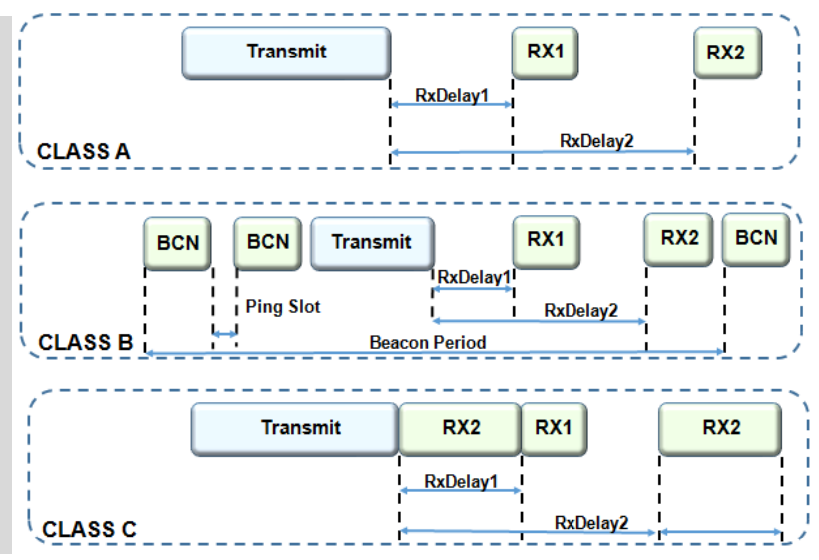
\includegraphics[width=0.6\textwidth]{07_lorawan}
